
\chapter{Labs with CVA6 Project}
\label{chapter:labs_with_cva6}


\begin{figure}[t]
    \centering
    \frame{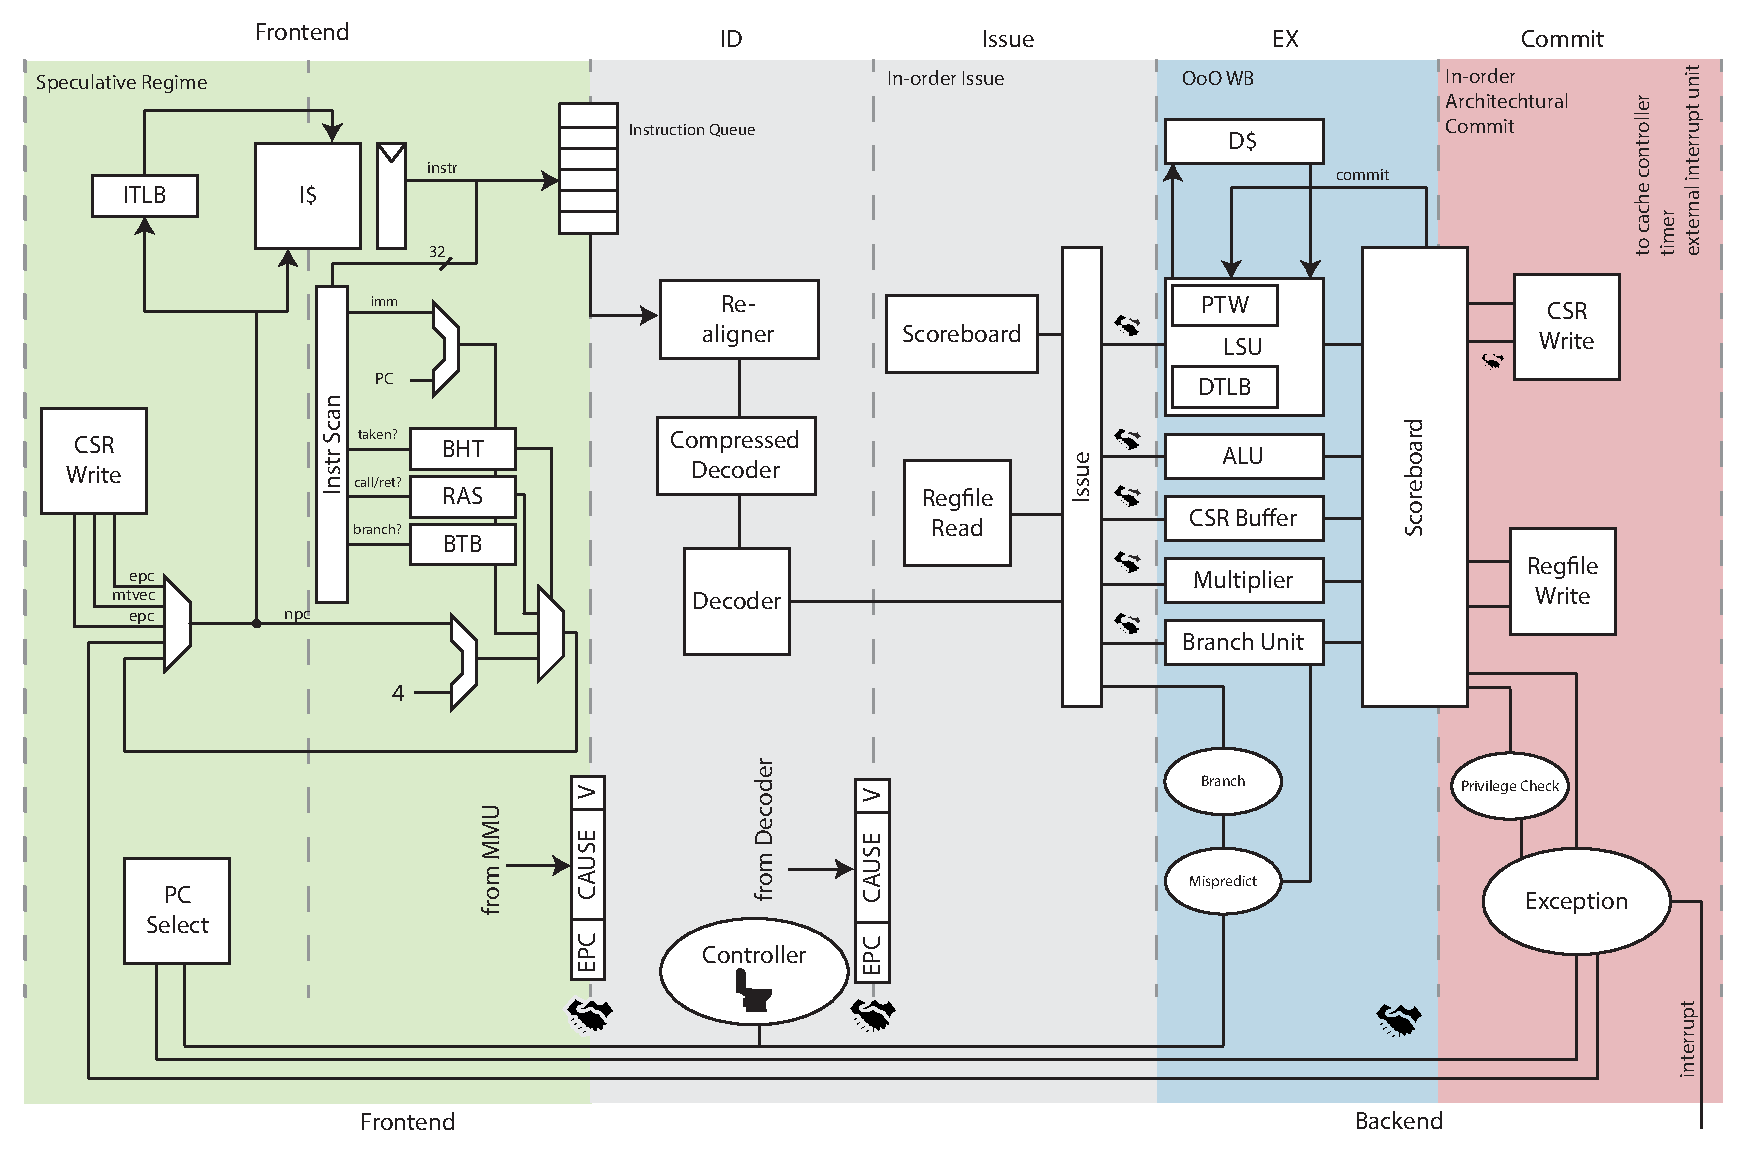
\includegraphics[width=0.7\linewidth]{media/cva6_overview.pdf}}
    \caption{CVA6 Block Diagram \cite{cva6}}
    \label{fig:cva6_overview}
\end{figure}


Standing as a culmination of all the Verilog education philosophies described in this thesis is a set of assignments I designed under the project label \enquote{Labs with CVA6}.
By drawing on my experiences from my time at Intel, my contributions to open-source projects, and interactions with industry contacts, I wrote four labs that aimed to give students practical experience with advanced computer architecture concepts.
Each lab is centered around the fully featured RISC-V core CVA6 \cite{cva6}, which is perfect for advanced architecture education due to its 6-stage pipeline, dynamic branch predictor, L1 cache, scoreboard unit, and virtual memory support (see \autoref{fig:cva6_overview}).
The labs presented students with a unique chance to engage with a fully-featured and transparent RISC-V core.
This hands-on interaction facilitated a deeper comprehension of important architectural principles while also enhancing their ability to work with large and complex SystemVerilog designs.
These labs are available for free under the BSD-3-Clause license \cite{labsWithCVA6}.

\FloatBarrier

\section{These labs provide hands-on exploration of architectural concepts.}


\begin{figure}[t]
    \centering
    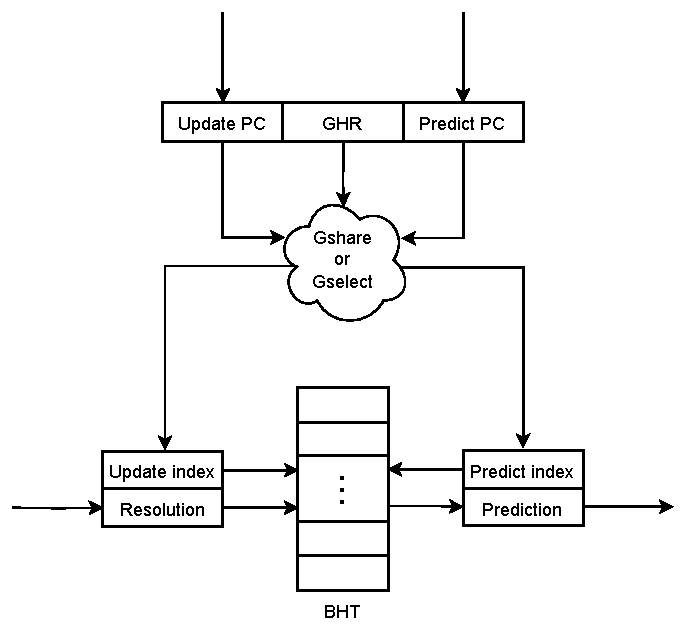
\includegraphics[width=0.8\linewidth]{media/graphics/labs_with_cva6/global_predictor.pdf}
    \caption[
        Branch Predictor Design for \enquote{Labs with CVA6}
    ]{
        Block diagram of the Global Two-Level Branch Predictor Design featured in \enquote{Labs with CVA6}.
        Participants are tasked with transforming CVA6's branch predictor into a more-sophisticated global predictor, enhancing the processor's performance by improving branch hit-rate for specifically designed benchmarks \cite{labsWithCVA6}.
    }
    \label{fig:branch_predictor}
\end{figure}


\begin{figure}[t]
    \centering
    \inputminted[frame=single]{systemverilog}{code/cache_lab/cache.svh}
    \caption{Snippet of ``Labs with CVA6'' cache lab starter code \cite{labsWithCVA6}}
    \label{fig:cache_lab}
\end{figure}


\begin{figure}[t]
    \centering

    \subfloat[
        RISC-V assembly that demonstrates out-of-order execution.
    ]{
        \begin{minipage}{0.9\textwidth}
            \large
            \inputminted{gas}{media/code/OoO.S}
        \end{minipage}
        \vspace{4pt}
    }
    \vspace{4pt}

    \subfloat[
        Screenshot of WaveForm.
        \emph{(Note: this figure omits redundant cycles to improve readability)}.
    ]{
        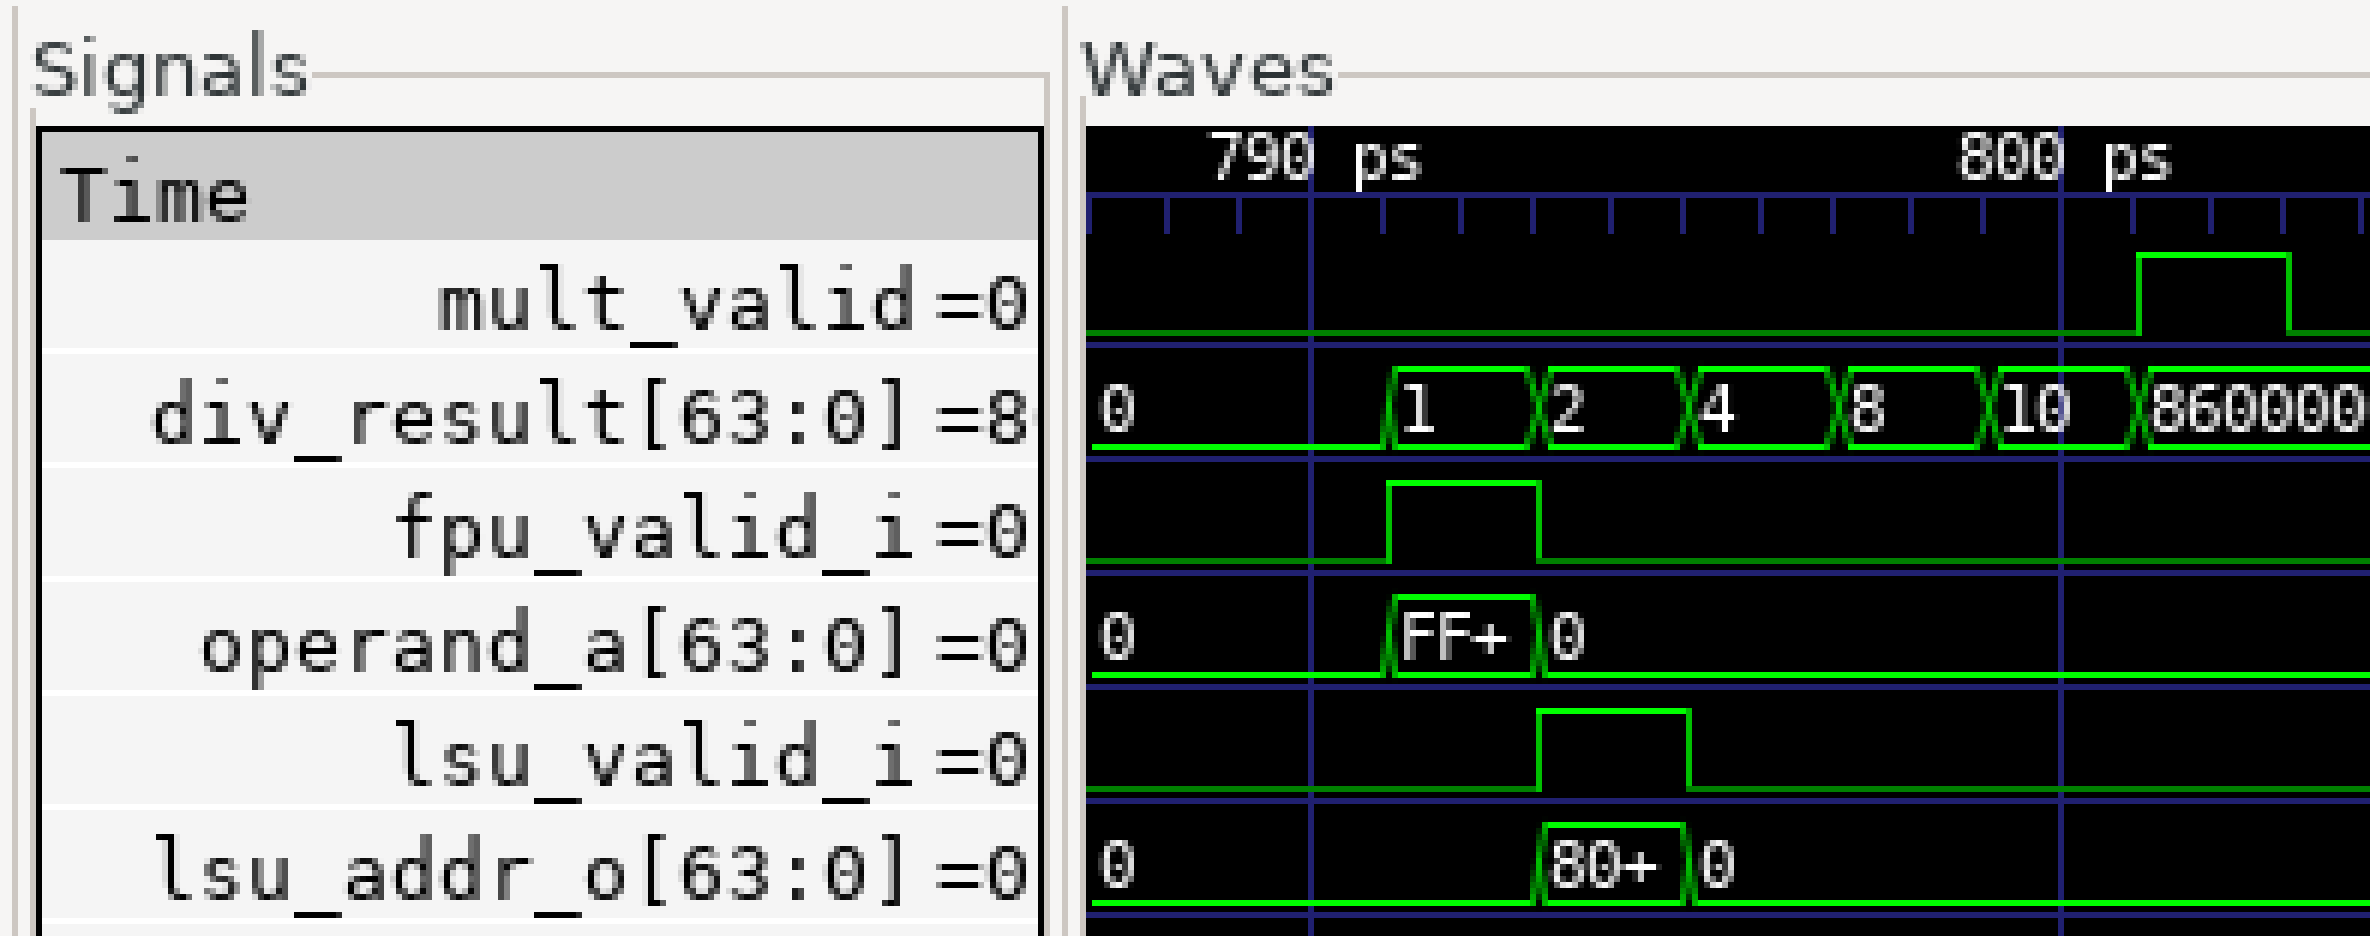
\includegraphics[width=0.9\linewidth]{media/graphics/labs_with_cva6/OoO.png}
    }
    \vspace{6pt}

    \caption[
        Out-of-Order Demonstration with CVA6
    ]{
        Out-of-Order Demonstration with CVA6: FPU and LSU finish before MULT \cite{SiffermanLatchUp}.
        In the Out-of-Order lab, participants are asked to write an assembly program to demonstrate code with and without different data-hazards.
    }
    \label{fig:OoO}

\end{figure}


\begin{figure}[t]
    \centering

    \subfloat[
        Digram provided to students to demonstrate how to move between privilege modes \cite{danielmangumRISCVPriv}.
    ]{
        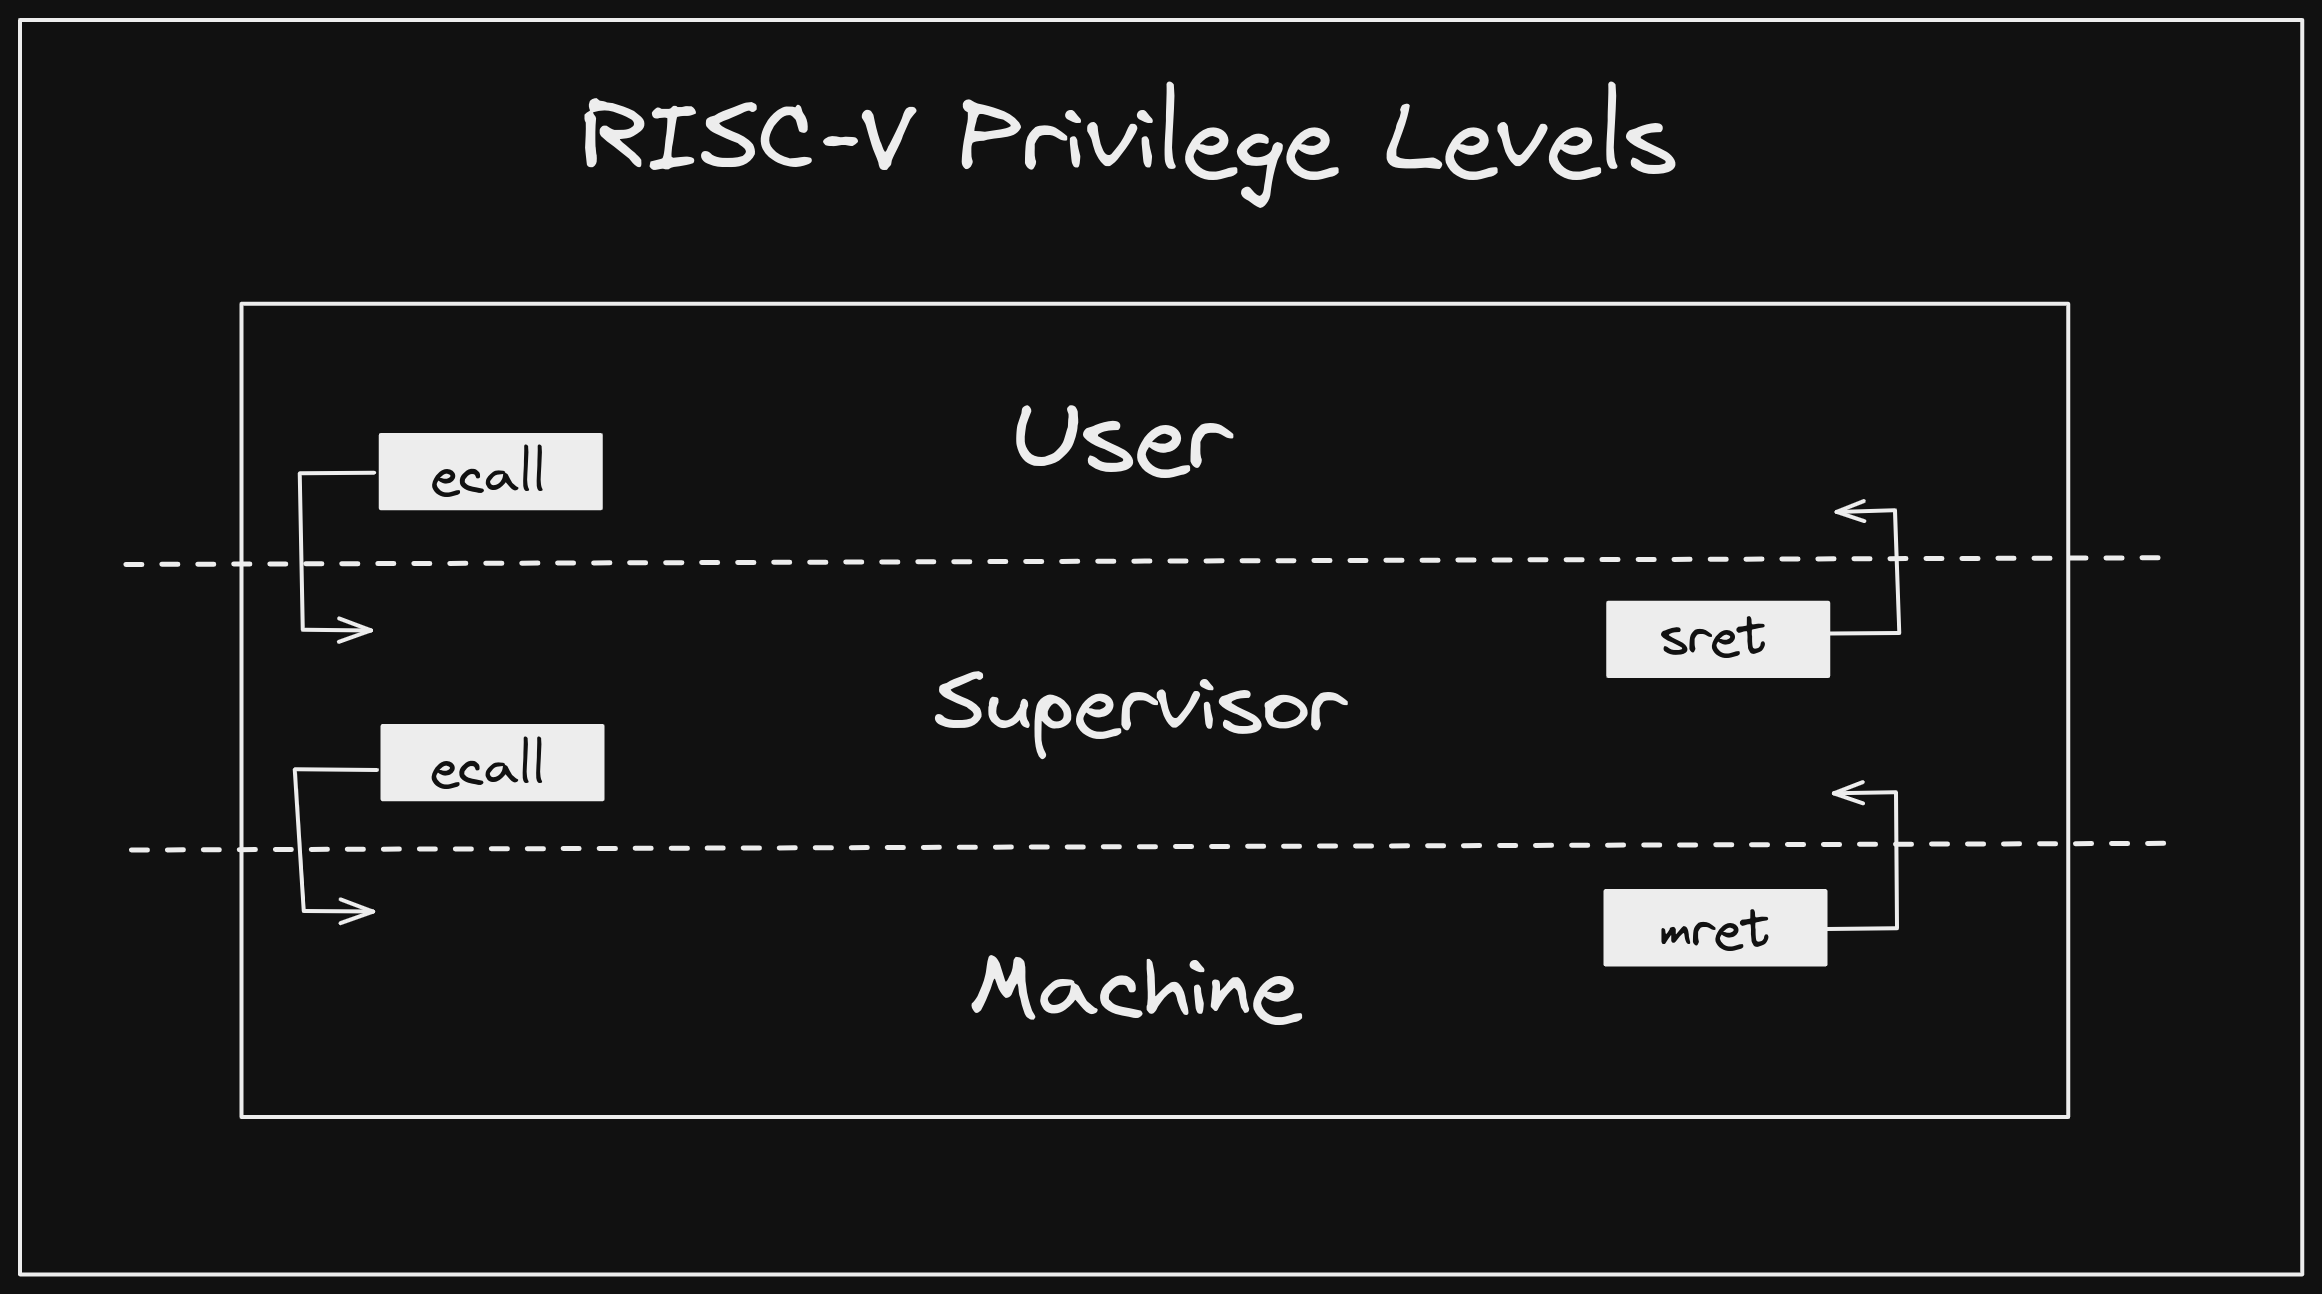
\includegraphics[width=0.8\linewidth]{media/graphics/labs_with_cva6/priv_levels.png}
    }

    \subfloat[
        Student drawing of a page table diagram
    ]{
        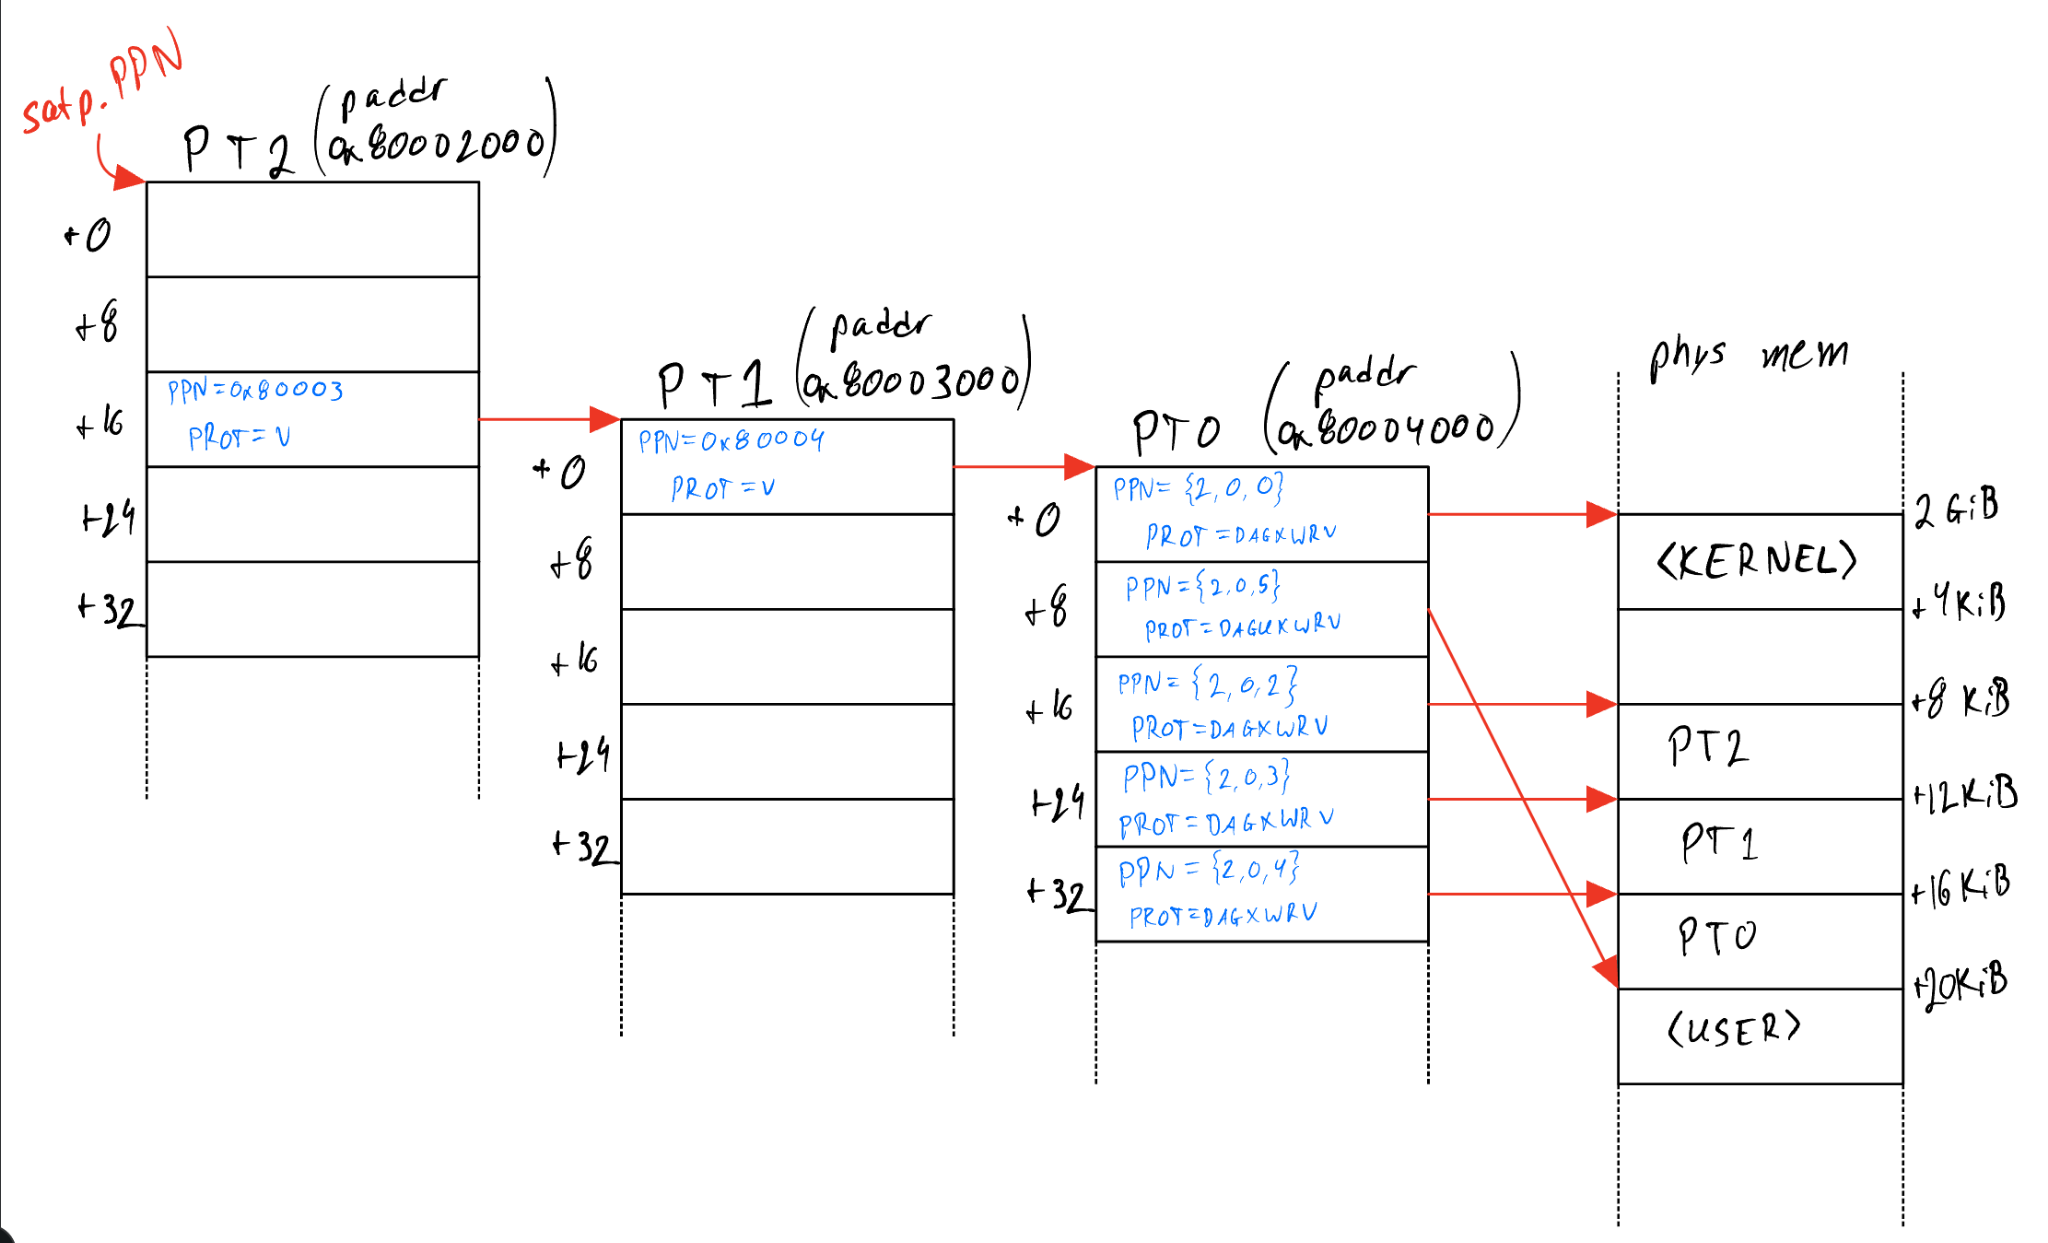
\includegraphics[width=0.8\linewidth]{media/graphics/labs_with_cva6/pt.png}
    }

    \caption[
        Virtual Memory Lab
    ]{
        Comparison of synthesis optimizations
    }
    \label{fig:virtual_memory}

\end{figure}


\enquote{Labs with CVA6} consists of four labs covering branch prediction, caching, out-of-order, and virtual memory.
The Branch Prediction Lab guides students in modifying the CVA6 testbench to display hit rate results and in adapting the CVA6 branch prediction unit RTL into a global predictor (see \autoref{fig:branch_predictor}).
Similarly, the Caching Lab asks students to write RTL for a victim-cache module, then requests the creation of assembly scripts that demonstrate CVA6's cache hierarchies and memory management (see \autoref{fig:cache_lab}).
Then moving away from custom RTL, in the Out-of-Order Lab, students further practice writing assembly to test their comprehension of out-of-order execution (see \autoref{fig:OoO}).
Finally, the Virtual Memory Lab enables students to configure privilege modes and add page-table entries by modifying a provided bootloader and OS (see \autoref{fig:virtual_memory}).
Based on ECE 154B student responses and post-lab discussions, it was evident that the practical insights offered by these labs substantially deepen understanding of the concepts.
The openness of CVA6's source code was pivotal to the labs' success, as it granted students the opportunity to interact with every implementation detail and feature of the core.
By studying open-source hardware designs, students can gain valuable and distinctive insights that traditional textbooks simply cannot provide.

\FloatBarrier

\section{There is high demand for hands-on learning experiences.}

Because \enquote{Labs with CVA6} is available under the BSD-3-Clause license, it has attracted attention from many non-ECE 154B audiences including instructors seeking to enrich their own architecture courses, researchers aiming to familiarize themselves with the specifics of CVA6, and SystemVerilog beginners eager to learn best practices.
In addition, I gave a well-appreciated talk about \enquote{Labs with CVA6} at \enquote{Latch-Up}, a conference hosted by The Free and Open Source Silicon Foundation \cite{SiffermanLatchUp}.
During my presentation, I expressed the practical and unique skills that students acquire through studying the code of well-verified, open-source designs.
This resonated deeply with several attendees, notably Rick O'Connor, the President and CEO at OpenHW Group, who notified me of the new OpenHW Group RISC-V core, CV-Wally \cite{cvwally}, that is designed as a supplemental codebase for the upcoming textbook, \enquote{RISC-V System-on-Chip Design}.
The popularity that \enquote{Labs with CVA6} has seen, and the recent creation of CV-Wally shows that there is strong demand for curriculums that offer transparency on implementation methods of real-world designs.
